\documentclass{article}
\usepackage{color}

%\usepackage{enumerate}
\usepackage{graphicx}
\usepackage{color}
\usepackage[cmex10]{amsmath}
\usepackage{array}
\usepackage{float}
\usepackage[utf8]{inputenc} 
\usepackage[portuguese]{babel}
\usepackage[font=normalsize,format=plain,labelfont=bf,up,textfont=up,figurename=Figura,tablename=Tabela]{caption}
\usepackage{subcaption}
\usepackage[top=1in, bottom=1in, left=1.25in, right=1.25in]{geometry}
\usepackage{indentfirst}
\usepackage{fancyhdr}

%% LaTeX Draw
%
%\usepackage[usenames,dvipsnames]{pstricks}
%\usepackage{epsfig}
%\usepackage{pst-grad} % For gradients
%\usepackage{pst-plot} % For axes
%\usepackage[space]{grffile} % For spaces in paths
%\usepackage{etoolbox} % For spaces in paths
%\makeatletter % For spaces in paths
%\patchcmd\Gread@eps{\@inputcheck#1 }{\@inputcheck"#1"\relax}{}{}
%\makeatother

% Font packages
\usepackage{amssymb}
\usepackage{amsfonts}
\usepackage{steinmetz}
% Nice extra font package, e.g. \mathds{1}
\usepackage{dsfont}


% Use multiple rows when writing tables
\usepackage{multirow}
\usepackage{booktabs}
\usepackage{bigstrut}
    \setlength\bigstrutjot{3pt}

% Uncomment next line to make footnots per page
\usepackage{perpage}

% Uncoment next group of lines to create the table of contents for the PDF
\usepackage{hyperref}
\definecolor{darkblue}{rgb}{0,0,0.5}
\hypersetup{
    pdftitle={Trabalho 1},
    pdfauthor={Gabriel Pelielo},
    bookmarksnumbered=true,     
    bookmarksopen=true,         
    bookmarksopenlevel=1,       
    colorlinks=true,
    linkcolor=darkblue,
    filecolor=darkblue,  
    urlcolor=darkblue,  
    citecolor=darkblue,              
    pdfstartview=Fit,           
    pdfpagemode=UseOutlines,    % this is the option you were lookin for
    pdfpagelayout=TwoPageRight
}

\renewcommand{\title}{Trabalho 2}
\newcommand{\subtitle}{Introdução à Otimização}
\pagestyle{fancy}
\fancyhead[L]{\title}
\fancyhead[R]{\subtitle}
\fancyhead[C]{\thepage}
\fancyfoot[C]{}

\allowdisplaybreaks

\renewcommand{\labelitemi}{\scalebox{0.8}[0.8]{$\bullet$}}
\newcommand{\tab}{\hspace{0.5cm}}

\definecolor{lightyellow}{rgb}{1,0.9568,0.8039}
\definecolor{mygreen}{rgb}{0, 0.35, 0}
\definecolor{myblue}{rgb}{0,0,1}

\begin{document}
\large
\begin{titlepage}
\begin{center}

% Upper part of the page. The '~' is needed because \\
% only works if a paragraph has started.

\includegraphics[width=0.15\textwidth]{logo.png}%~\\[0.5cm]

% Title
\rule{\linewidth}{0.5mm} \\[0.4cm]
{ \huge \bfseries \title \\[0.4cm] }
\rule{\linewidth}{0.5mm} \\[0.5cm]

\textsc{\Large \subtitle}\\[1.5cm]

% Author and supervisor
\begin{minipage}{0.4\textwidth}
\begin{flushleft} \large
\textbf{Alunos: \newline Cayo Valsamis \newline Gabriel Pelielo \newline Rafael Accácio \newline Rodrigo Moysés}\\
%NOME DOS ALUNOS

\end{flushleft}
\end{minipage}
\begin{minipage}{0.4\textwidth}
\begin{flushright} \large
\textbf{Professor:\newline Afonso Celso del Nero \newline \newline \newline} \\
%NOME DO PROFESSOR
\end{flushright}
\end{minipage}

\vfill

% Bottom of the page
{\large \today}

\end{center}
\end{titlepage}

\tableofcontents

\newpage

\section{Introdução}

O trabalho detalhado neste relatório se baseia em analisar métodos numéricos para realizar busca de mínimos de funções vetoriais. Foram implementados cinco métodos diferentes de localização de mínimos:

\begin{itemize}
	\item Método da Descida Máxima (ou gradiente)
	\item Método do Gradiente Conjugado
	\item Método de Newton
	\item Método de Newton Modificado
	\item Método de Quase Newton
\end{itemize}

Todos os métodos foram implementados na plataforma \textit{MATLAB}, através de um programa de interface gráfica usado para escolher o método desejado e inserir alguns valores necessários para executar a busca. O objetivo do trabalho foi comparar esses métodos de acordo com os quesitos de tempo de execução, número necessário de iterações e por fim qualificá-los de acordo com cada função inserida.

\section{Método de Fibonacci}\label{sec:fibo}

bla bla bla

\section{Método da Divisão Áurea}\label{sec:aurea}

O método da Divisão áurea é outro método de localização de mínimos de funções escalares. Foi criado como uma avanço para o método de Fibonacci e se baseia na razão áurea. Por definição, para dividir o segmento de reta da figura \ref{fig:abc} na razão áurea, é necessário que

\begin{equation*}
\dfrac{\overline{AC}}{\overline{AB}} = \dfrac{\overline{AB}}{\overline{BC}}
\end{equation*}

\begin{figure}[h]
	\begin{center}
		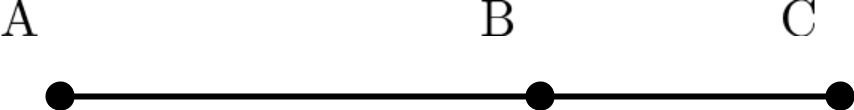
\includegraphics[width=8cm]{../aurea/dots_a_b_c.png}   
		\caption{Segmento de reta $ \overline{ABC} $}
		\label{fig:abc}
	\end{center}
\end{figure}

Dessa relação, podemos deduzir que $ \overline{AB} = 0.618\overline{AC} $. Assim, o segmento de reta fica dividido segundo a razão áurea, como mostra a figura \ref{fig:aurea_abc}.

\begin{figure}[h]
	\begin{center}
		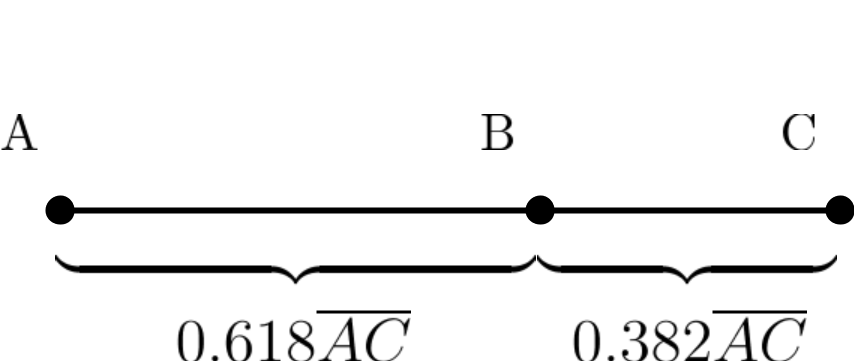
\includegraphics[width=8cm]{../aurea/dots_a_b_c_aurea.png}   
		\caption{Divisão áurea do segmento de reta}
		\label{fig:aurea_abc}
	\end{center}
\end{figure}

A sequência de Fibonacci, base para a construção do método de Fibonacci, tem uma semelhança com a razão áurea: A divisão entre dois números consecutivos dessa sequência converge para a razão áurea. Ou seja, o método da divisão áurea tenta aprimorar o método de Fibonacci porque desde a primeira iteração, já faz a divisão do intervalo para o melhor possível.

\begin{figure}[h]
	\begin{center}
		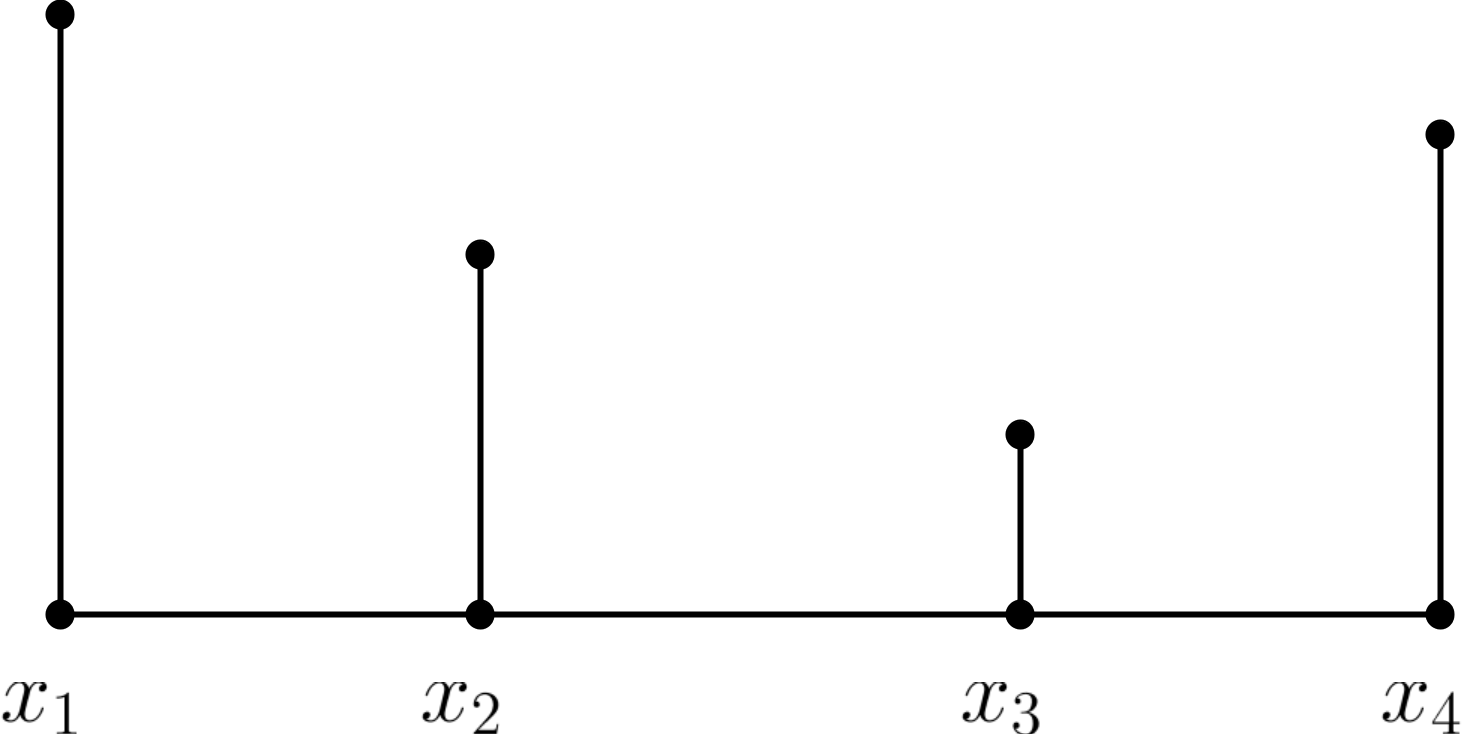
\includegraphics[width=8cm]{../aurea/aurea_fx.png}   
		\caption{Divisão áurea do segmento de reta}
		\label{fig:aurea_fx}
	\end{center}
\end{figure}

A figura \ref{fig:aurea_fx} ilustra a execução do método. É definido um intervalo que vai de $ x_1 $ até $ x_4 $ e dentro desse intervalo são escolhidos mais dois pontos, $ x_2 $ e $ x_3 $, porém dessa vez com a regra de divisão áurea. Depois disso, são calculados os valores da função objetivo que se deseja minimizar para os quatro pontos.

Tendo os dois valores $ f(x_2) $ e $ f(x_3) $, é selecionado o maior deles e o intervalo adjacente à esse é retirado. No caso da figura \ref{fig:aurea_fx}, o ponto $ x_1 $ seria retirado. Para continuar o método, é necessário que mais um ponto seja adicionado, novamente com a regra da razão áurea. Agora que temos novamente 4 pontos, o método pode ser repetido até que uma tolerância escolhida tenha sido atingida, e assim é localizado o mínimo da função.

Com o algoritmo da divisão áurea construído, foram testadas quatro funções para efeitos de comparação:

\begin{itemize}
	\item $ f_1(x) = 3x^2 + 20x - 8 $
	\item $ f_2(x) = xsin(x)cos(x) $
	\item $ f_3(x) = 5x $
	\item $ f_4(x) = -e^{-\mid x \mid} $
\end{itemize}

\newpage

Os resultados para a função $ f_1(x) $ foram:

\begin{figure}[h]
	\begin{center}
		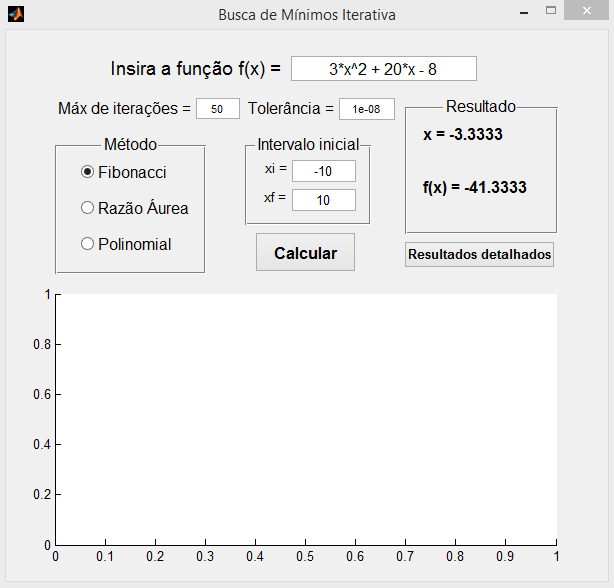
\includegraphics[width=14cm]{../aurea/f1_gui.png}   
		\caption{Janela de inicialização de $ f_1(x) $}
		\label{fig:f1_gui}
	\end{center}
\end{figure}

\begin{figure}[h!]
	\begin{center}
		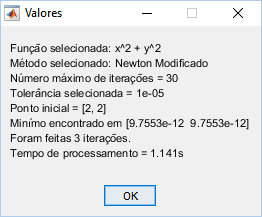
\includegraphics[width=6cm]{../aurea/f1_resultados.png}   
		\caption{Resultados detalhados de $ f_1(x) $}
		\label{fig:f1_resultados}
	\end{center}
\end{figure}

Os resultados para a função $ f_2(x) $ foram:

\begin{figure}[h]
	\begin{center}
		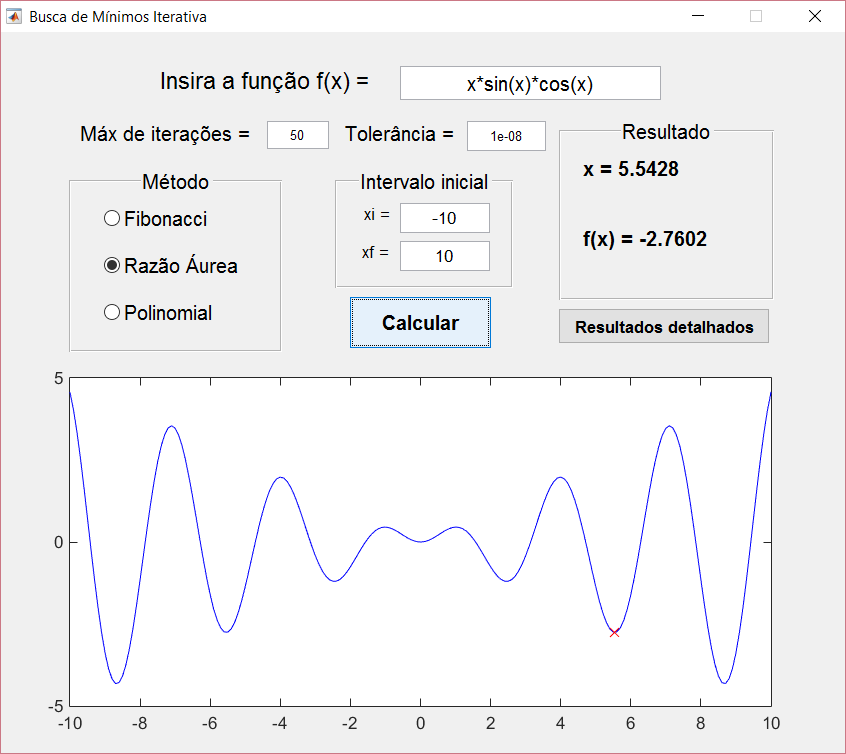
\includegraphics[width=14cm]{../aurea/f2_gui.png}   
		\caption{Janela de inicialização de $ f_2(x) $}
		\label{fig:f2_gui}
	\end{center}
\end{figure}

\begin{figure}[h!]
	\begin{center}
		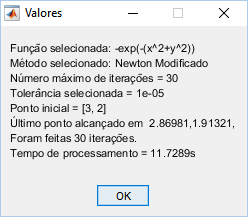
\includegraphics[width=6cm]{../aurea/f2_resultados.png}   
		\caption{Resultados detalhados de $ f_2(x) $}
		\label{fig:f2_resultados}
	\end{center}
\end{figure}

Os resultados para a função $ f_3(x) $ foram:

\begin{figure}[h]
	\begin{center}
		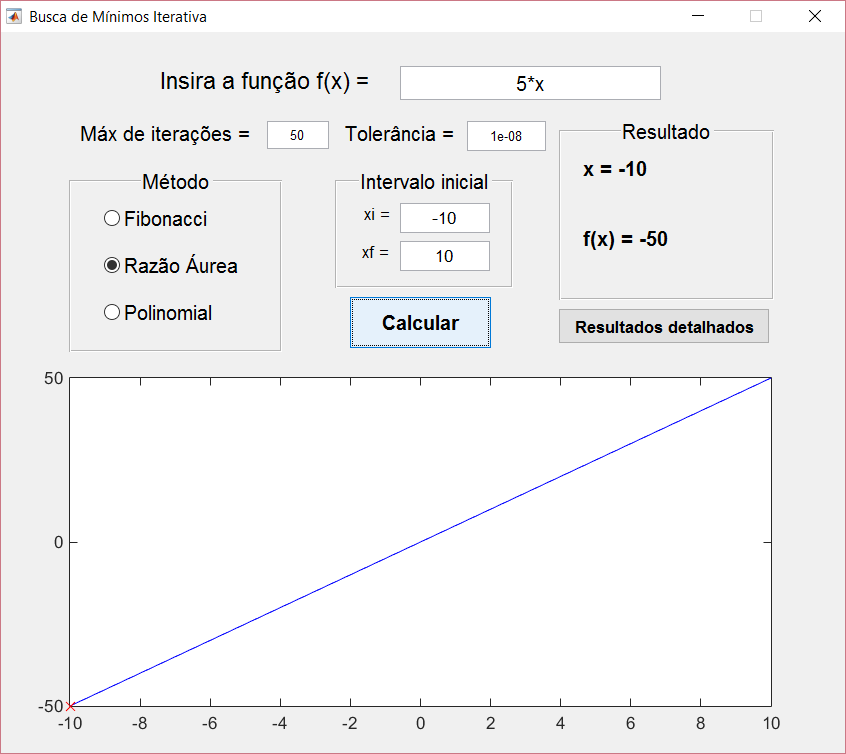
\includegraphics[width=14cm]{../aurea/f3_gui.png}   
		\caption{Janela de inicialização de $ f_3(x) $}
		\label{fig:f3_gui}
	\end{center}
\end{figure}

\begin{figure}[h!]
	\begin{center}
		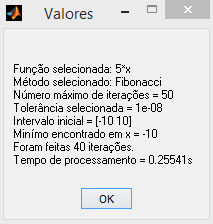
\includegraphics[width=6cm]{../aurea/f3_resultados.png}   
		\caption{Resultados detalhados de $ f_3(x) $}
		\label{fig:f3_resultados}
	\end{center}
\end{figure}

Os resultados para a função $ f_4(x) $ foram:

\begin{figure}[h]
	\begin{center}
		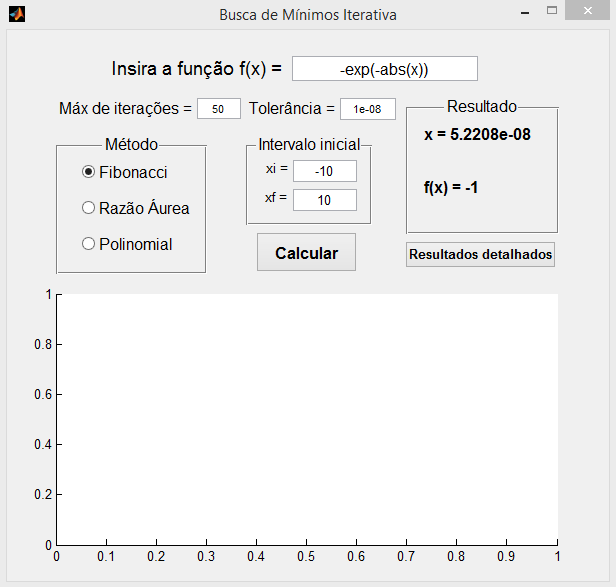
\includegraphics[width=14cm]{../aurea/f4_gui.png}   
		\caption{Janela de inicialização de $ f_4(x) $}
		\label{fig:f4_gui}
	\end{center}
\end{figure}

\begin{figure}[h!]
	\begin{center}
		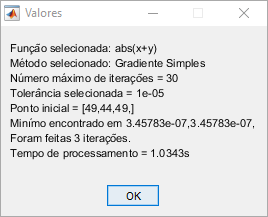
\includegraphics[width=6cm]{../aurea/f4_resultados.png}   
		\caption{Resultados detalhados de $ f_4(x) $}
		\label{fig:f4_resultados}
	\end{center}
\end{figure}


\section{Método da Interpolação Polinomial}\label{sec:interpol}

O método de Interpolação Polinomial é mais um método numérico iterativo para minimização de funções. 

\begin{figure}[h]
	\begin{center}	
		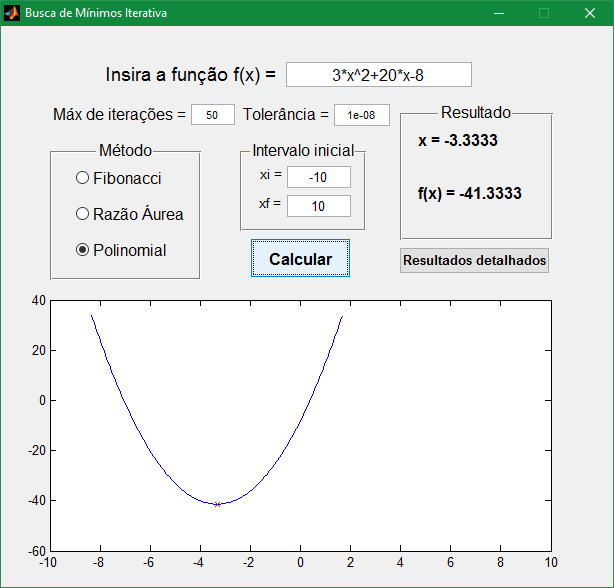
\includegraphics[width=14cm]{../interpol/f1_gui.PNG}
		\caption{escrevaaquiseucaption}
		\label{fig:f1_gui}
	\end{center}
\end{figure}

\begin{figure}[H]
	\begin{center}	
		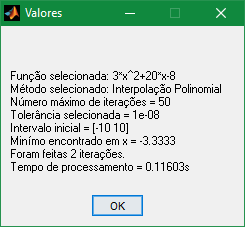
\includegraphics[width=6cm]{../interpol/f1_resultados.PNG}
		\caption{escrevaaquiseucaption}
		\label{fig:f1_resultados}
	\end{center}
\end{figure}

\begin{figure}[H]
	\begin{center}	
		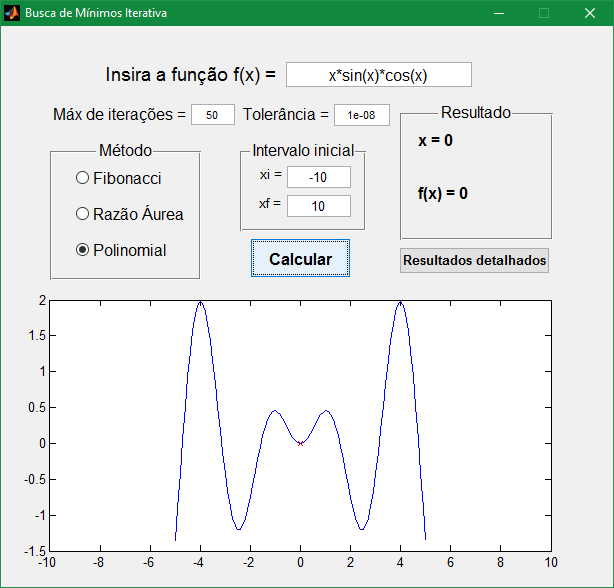
\includegraphics[width=14cm]{../interpol/f2_gui.PNG}
		\caption{escrevaaquiseucaption}
		\label{fig:f2_gui}
	\end{center}
\end{figure}

\begin{figure}[H]
	\begin{center}	
		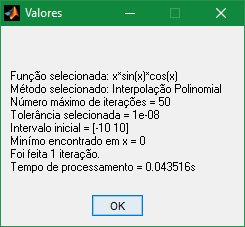
\includegraphics[width=6cm]{../interpol/f2_resultados.PNG}
		\caption{escrevaaquiseucaption}
		\label{fig:f2_resultados}
	\end{center}
\end{figure}

\begin{figure}[H]
	\begin{center}	
		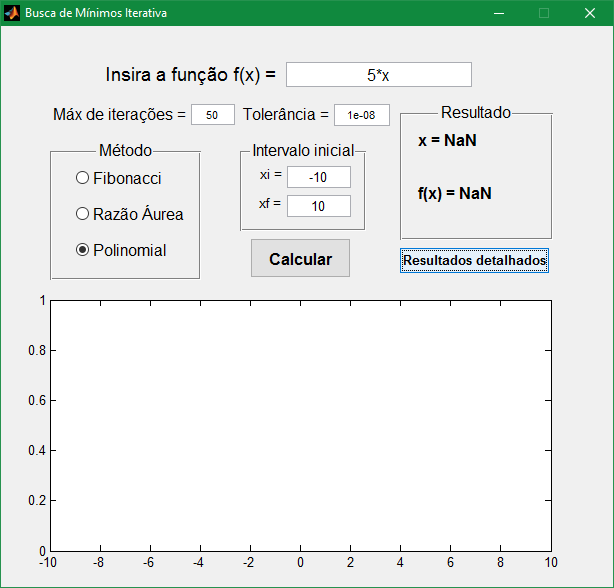
\includegraphics[width=14cm]{../interpol/f3_gui.PNG}
		\caption{escrevaaquiseucaption}
		\label{fig:f3_gui}
	\end{center}
\end{figure}

\begin{figure}[H]
	\begin{center}	
		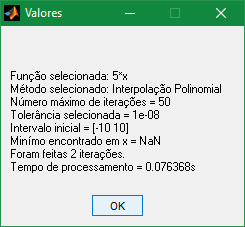
\includegraphics[width=6cm]{../interpol/f3_resultados.PNG}
		\caption{escrevaaquiseucaption}
		\label{fig:f3_resultados}
	\end{center}
\end{figure}

\begin{figure}[H]
	\begin{center}	
		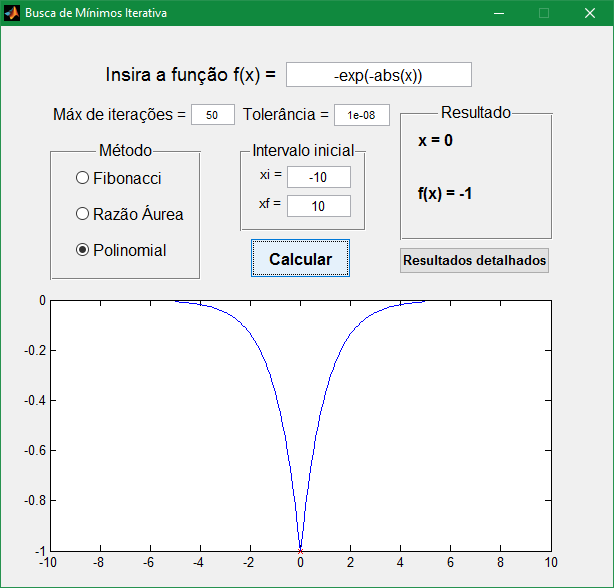
\includegraphics[width=14cm]{../interpol/f4_1_gui.PNG}
		\caption{escrevaaquiseucaption}
		\label{fig:f4_1_gui}
	\end{center}
\end{figure}

\begin{figure}[H]
	\begin{center}	
		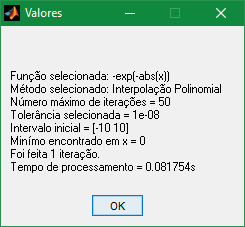
\includegraphics[width=6cm]{../interpol/f4_1_resultados.PNG}
		\caption{escrevaaquiseucaption}
		\label{fig:f4_1_resultados}
	\end{center}
\end{figure}

\begin{figure}[H]
	\begin{center}	
		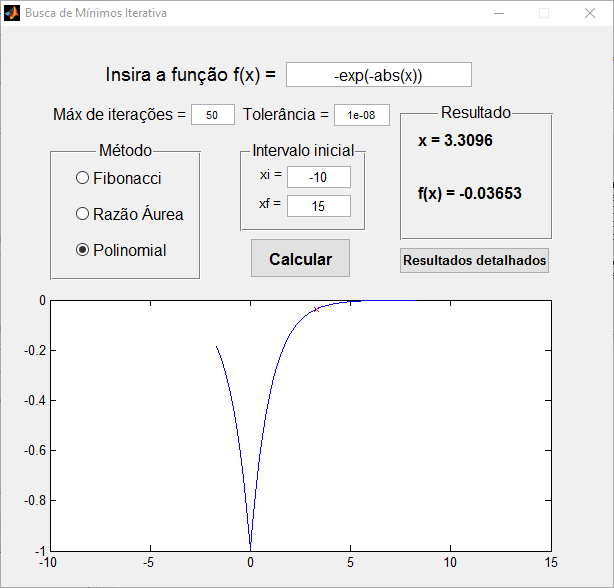
\includegraphics[width=14cm]{../interpol/f4_2_gui.PNG}
		\caption{escrevaaquiseucaption}
		\label{fig:f4_2_gui}
	\end{center}
\end{figure}

\begin{figure}[H]
	\begin{center}	
		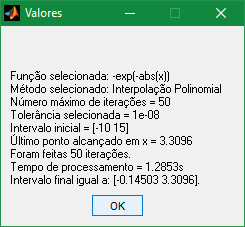
\includegraphics[width=6cm]{../interpol/f4_2_resultados.PNG}
		\caption{escrevaaquiseucaption}
		\label{fig:f4_2_resultados}
	\end{center}
\end{figure}



\section{Interface Gráfica}\label{sec:gui}

bla bla bla

\section{Conclusão}

bla bla bla
	
%\textcolor{mygreen}{text} - Dá cor verde ao texto
%\textcolor{myblue}{text}  - Dá cor azul  ao texto


\end{document}